\documentclass{standalone}
\usepackage{tikz}
\usetikzlibrary{patterns, calc}

\begin{document}
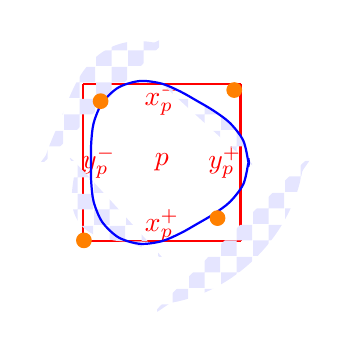
\begin{tikzpicture}
    % Define the main pixel 'p'
    \coordinate (p) at (0,0);
    \node[red] at (p) {$p$};
    
    % Define the x and y boundaries
    \draw[red, thick] ($(p) + (-1, 1)$) -- ($(p) + (-1, -1)$);
    \draw[red, thick] ($(p) + (1, 1)$) -- ($(p) + (1, -1)$);
    \draw[red, thick] ($(p) + (-1, 1)$) -- ($(p) + (1, 1)$);
    \draw[red, thick] ($(p) + (-1, -1)$) -- ($(p) + (1, -1)$);
    
    % Label the boundaries
    \node[red] at ($(p) + (0, 0.8)$) {$x_p^{-}$};
    \node[red] at ($(p) + (0, -0.8)$) {$x_p^{+}$}; % corrected label placement
    \node[red] at ($(p) + (0.8, 0)$) {$y_p^{+}$}; % corrected label placement
    \node[red] at ($(p) + (-0.8, 0)$) {$y_p^{-}$}; % corrected label placement
    
    % Draw the irregular region with checkered pattern
    \fill[pattern=checkerboard,pattern color=blue!10] 
        plot[domain=0:90,smooth cycle] (xy polar cs:angle=\x,radius= {1+0.1*cos(3*\x)});
    \fill[pattern=checkerboard,pattern color=blue!10] 
        plot[domain=90:180,smooth cycle] (xy polar cs:angle=\x,radius= {1.5+0.1*sin(4*\x)});
    \fill[pattern=checkerboard,pattern color=blue!10] 
        plot[domain=180:270,smooth cycle] (xy polar cs:angle=\x,radius= {1.2+0.1*cos(5*\x)});
    \fill[pattern=checkerboard,pattern color=blue!10] 
        plot[domain=270:360,smooth cycle] (xy polar cs:angle=\x,radius= {1.8+0.1*sin(2*\x)});
    
    % Draw the blue boundary (simplified representation)
    \draw[blue, thick] plot[domain=0:360,smooth cycle] (xy polar cs:angle=\x,radius= {1+0.1*cos(3*\x)});
    
    % Orange points
    \fill[orange] (135:1.1) circle (0.1);
    \fill[orange] (225:1.4) circle (0.1);
    \fill[orange] (315:1.0) circle (0.1);
    \fill[orange] (45:1.3) circle (0.1);
    
\end{tikzpicture}
\end{document}